
\chapter{Rezultate teoretice și experimentale}
\label{cap:rezultate}

% Împreună cu partea de prezentare a proiectului, trebuie să reprezinte aproximativ 70\% din lucrare. 

% Aici sunt prezentate metodele teoretice sau practice de validare/verificare a soluțiilor propuse în partea anterioară, scenariile de testare a corectitudinii funcționale, a utilizabilității, performanței etc.  

% De asemenea, rezultatele testelor experimentale se pretează unor interpretări și comparații cu rezultatele altor metode similare. 

În acest capitol se prezintă metoda utilizată pentru validarea funcțională și evaluarea performanțelor sistemului de compilare distribuită
dezvoltat. Prima parte descrie aspecte legate de mediul de rulare care a fost creat pentru desfășurarea testelor, precum 
configurația hardware și software a nodurilor ce fac parte din sistem, dar și modul în care acestea sunt conectate.

Ulterior, sunt prezentate rezultatele obținute în urma compilării distribuite  a unor proiecte open-source reprezentative, dezvoltate
în limbajele C sau C++. Se compilează aplicații reale, cu dimensiuni și structuri diferite ale proiectului, pentru a permite evaluarea
comportamentului sistemului în condiții de utilizare practică. Metrica principală de evaluare o reprezintă timpul final de compilare și
îmbunătățirea duratei de build comparativ cu compilarea locală.

\section{Structura mediului de rulare}

Pentru testarea sistemului au a fost creat un mediu de evaluare alcătuit din trei noduri fizice: un sistem desktop și două
laptop-uri. Configurația a fost aleasă cu scopul de a reproduce un scenariu realist de utilizare, în care mai multe sisteme de calcul 
plasate în aceeași rețea locală își partajează resursele computaționale pentru a executa sarcinile de compilare mai rapid.

Cele trei sisteme au fost conectate în cadrul aceleiași rețele locale LAN, utilizând conexiuni Ethernet pentru a se conecta la
un switch Gigabit Ethernet central. Am optat pentru crearea unei infrastructuri de comunicație prin cablu Ethernet pentru a elimina
variațiile de latență și de lungime de bandă întâlnite la comunicarea prin WiFi. Astfel, putem evalua doar performanțele sistemului
dezvoltat, fără a lua în calcul influența mediului de transmisie.

Pe parcursul experimentelor, unul dintre sisteme a jucat rolul de client, fiind responsabil pentru inițierea operațiunilor de compilare,
iar celelalte două sisteme rămase au fost configurate ca noduri pentru compilare, care deservesc solicitările clientului și returnează
rezultatele compilării către acesta.

Pentru a menține omogenitatea mediilor de rulare și a elimina potențialele diferențe de versiune, toate cele trei sisteme de test 
au fost configurate să ruleze aceeași distribuție de Linux, \textbf{Ubuntu 24.04}. Pentru compilarea proiectelor de test se utilizează
compilatoarele \textbf{GCC} și \textbf{G++} cu versiunea \textbf{13.3.0}.

Cele trei sisteme folosite pentru teste au următoarele configurații hardware:

\begin{itemize}
    \item Sistem desktop:
    \begin{itemize}
        \item Procesor Intel I7-4790 cu 4 nuclee și 8 thread-uri @ 3.60 GHz
        \item 16 GB memorie RAM
    \end{itemize}
    \item Primul laptop:
    \begin{itemize}
        \item Procesor Intel I5-1335U cu 10 nuclee și 12 thread-uri @ 4.0 GHz
        \item 16 GB memorie RAM
    \end{itemize}
    \item Al doilea laptop:
    \begin{itemize}
        \item Procesor AMD Ryzen 7 3700U cu 4 nuclee și 8 thread-uri @ 4.0 GHz
        \item 16 GB memorie RAM
    \end{itemize}
\end{itemize}


Figura \ref{fig:network_topology} ilustrează structura mediului de rulare, cu cele trei sisteme de calcul conectate folosind un switch central Gigabit Ethernet.

\begin{figure}[H]
    \centering
    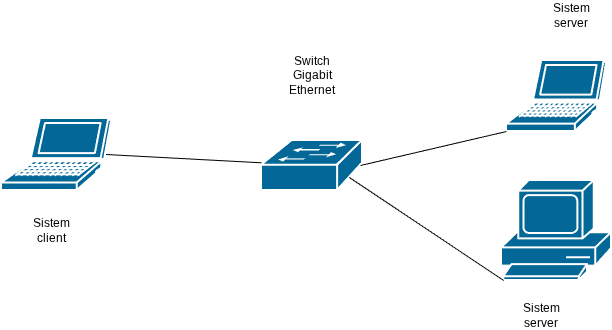
\includegraphics[width=0.65\linewidth, height=0.4\linewidth]{figures/network_topology.png}
    \caption{Topologia rețelei sistemului de compilare distribuită}
    \label{fig:network_topology}
\end{figure}

\newpage
